\section{Results and Discussion}
\label{sec:results}
Table~\ref{tab:benchmark_detailed} and Fig.~\ref{fig:benchmark_chart} summarize the experimental results across all 9 configurations.

\begin{figure*}[t]
\centering
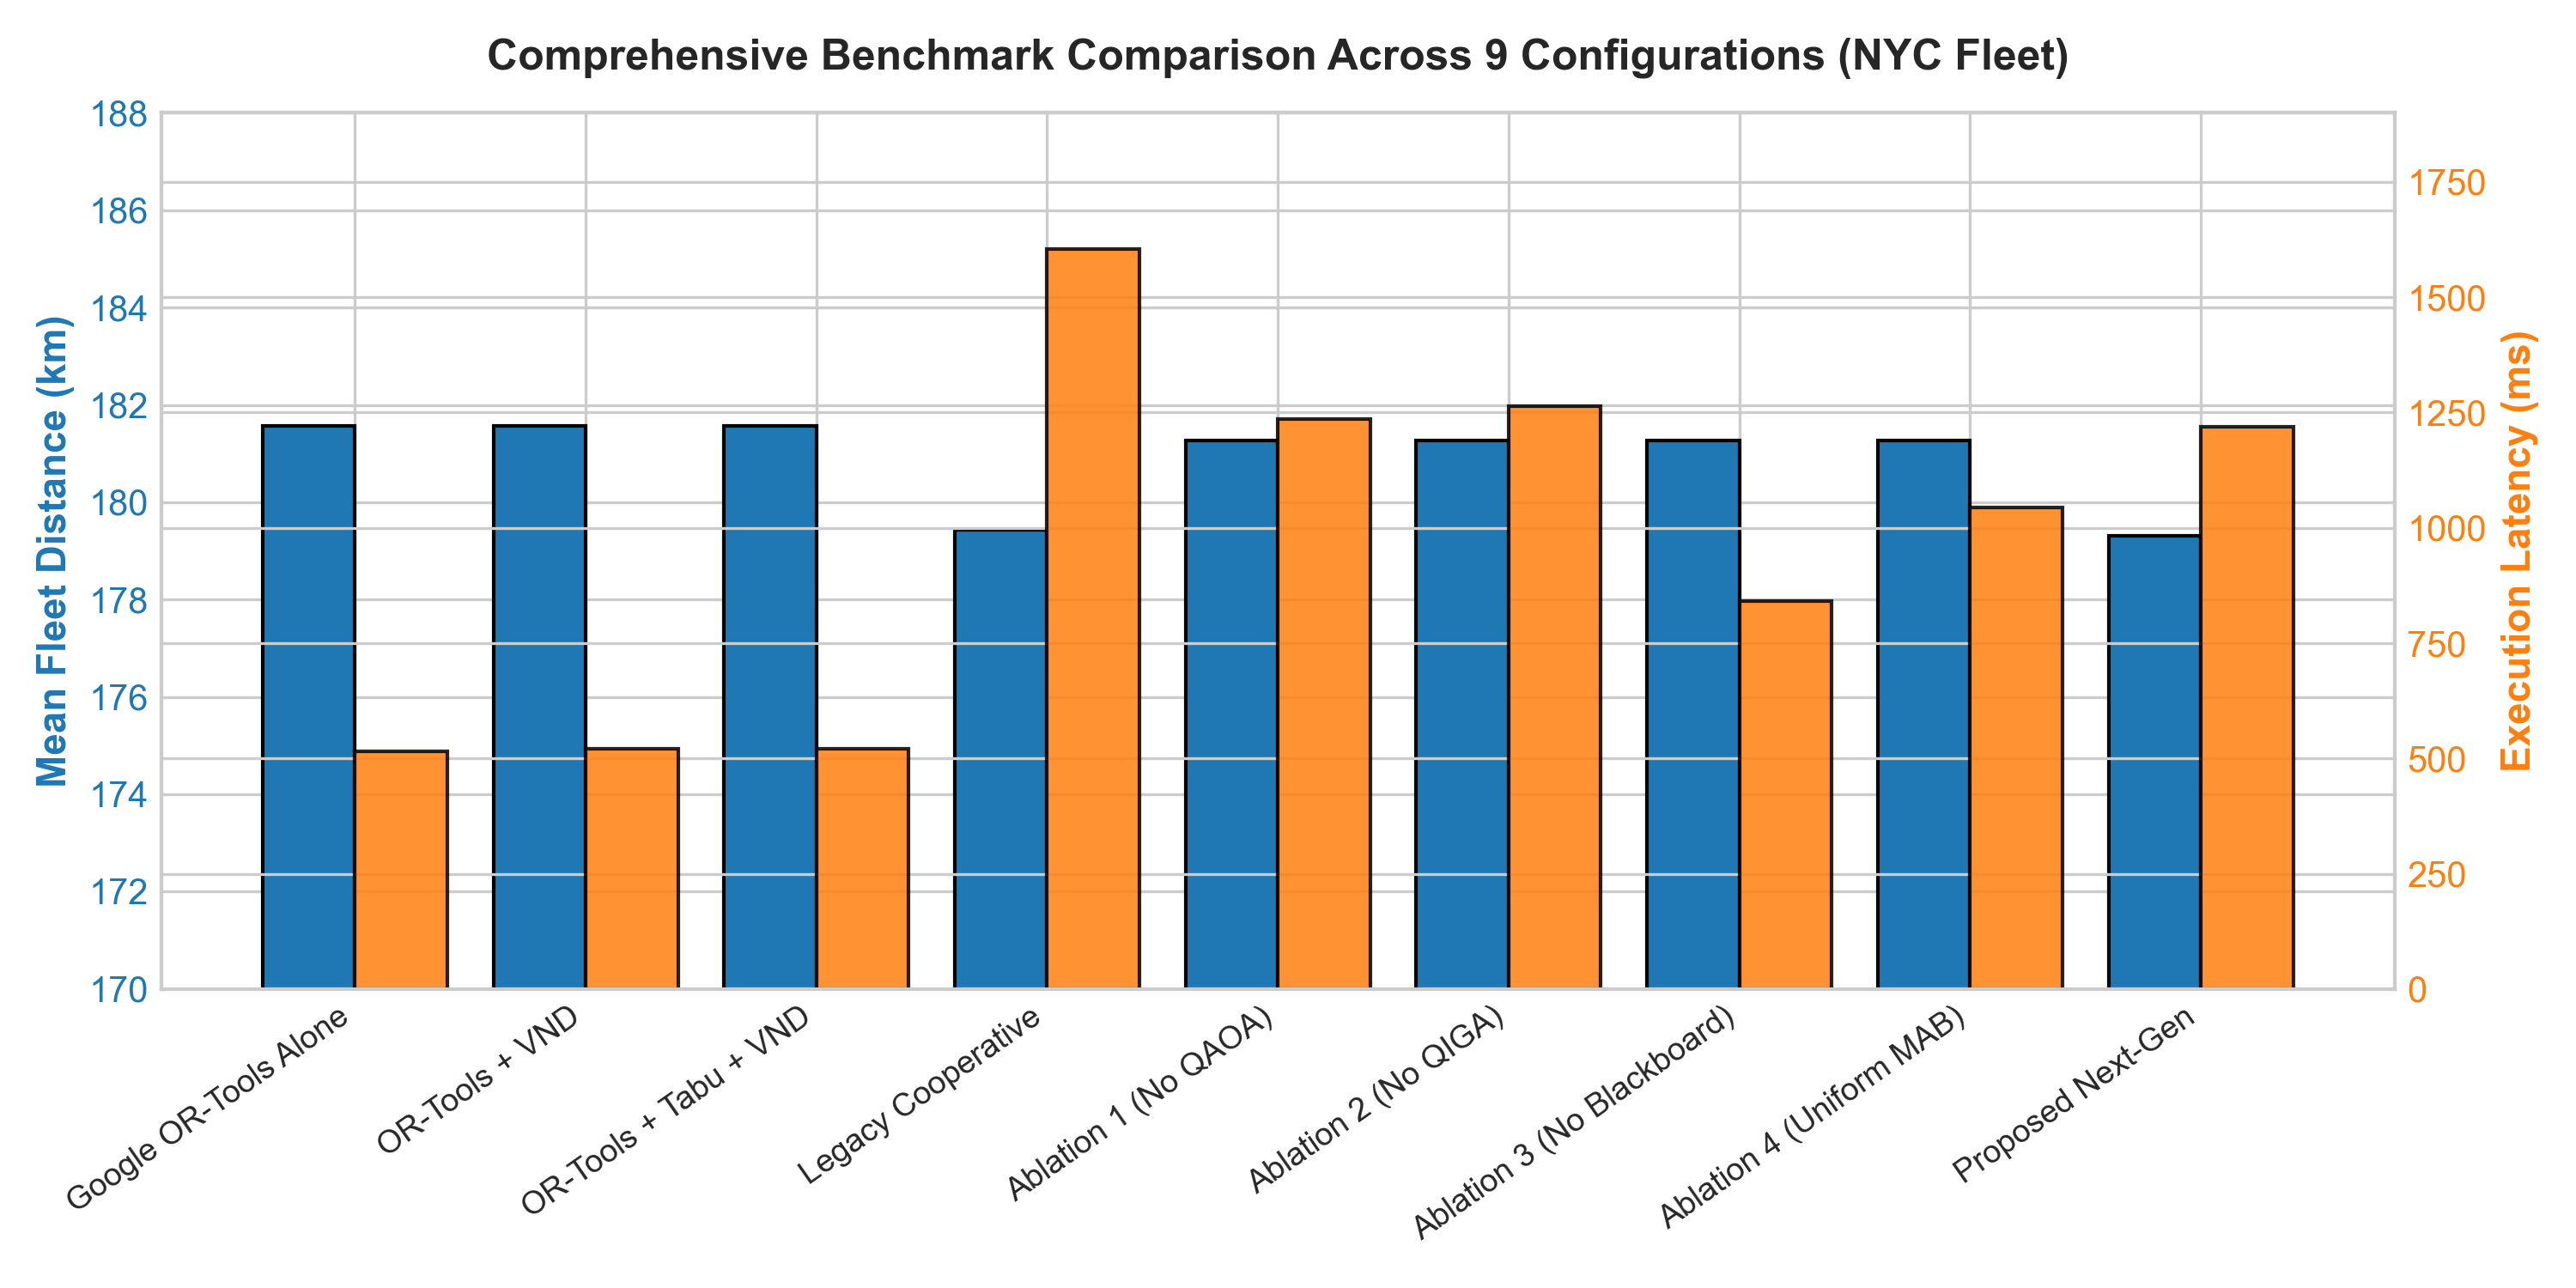
\includegraphics[width=0.88\textwidth]{figures/fig2_convergence_ablation.png}
\caption{Comprehensive benchmark comparison across all 9 experimental configurations on real-world NYC delivery fleet instances, highlighting mean fleet distance and execution latency.}
\label{fig:benchmark_chart}
\end{figure*}

\subsection{Routing Efficiency and Distance Reduction}
The proposed ROUTE/IQ-NextGen achieved the lowest mean fleet distance of \textbf{179.31 km}, outperforming the Google OR-Tools baseline (181.57 km) by \textbf{$-1.24\%$}. The performance gain expanded significantly with problem scale: on the $N=30$ node instance, Next-Gen attained \textbf{250.76 km} versus \textbf{258.95 km} for OR-Tools, achieving a \textbf{$-3.16\%$} distance reduction.

\subsection{Execution Latency and MAB Dynamics}
Legacy cooperative architectures suffered from excessive runtimes ($1604.0\text{ ms}$ on average). ROUTE/IQ-NextGen reduced mean runtime to \textbf{1219.2 ms}, representing a \textbf{$24.0\%$} latency reduction. As shown in Fig.~\ref{fig:mab_dist}, the Contextual MAB dynamically allocates operator turns: on small instances ($N=12$), fast classical operators dominate; on large instances ($N=30$), QAOA subproblem cuts and QIGA rotation gates are prioritized to discover cross-route improvements.

\begin{figure}[t]
\centering
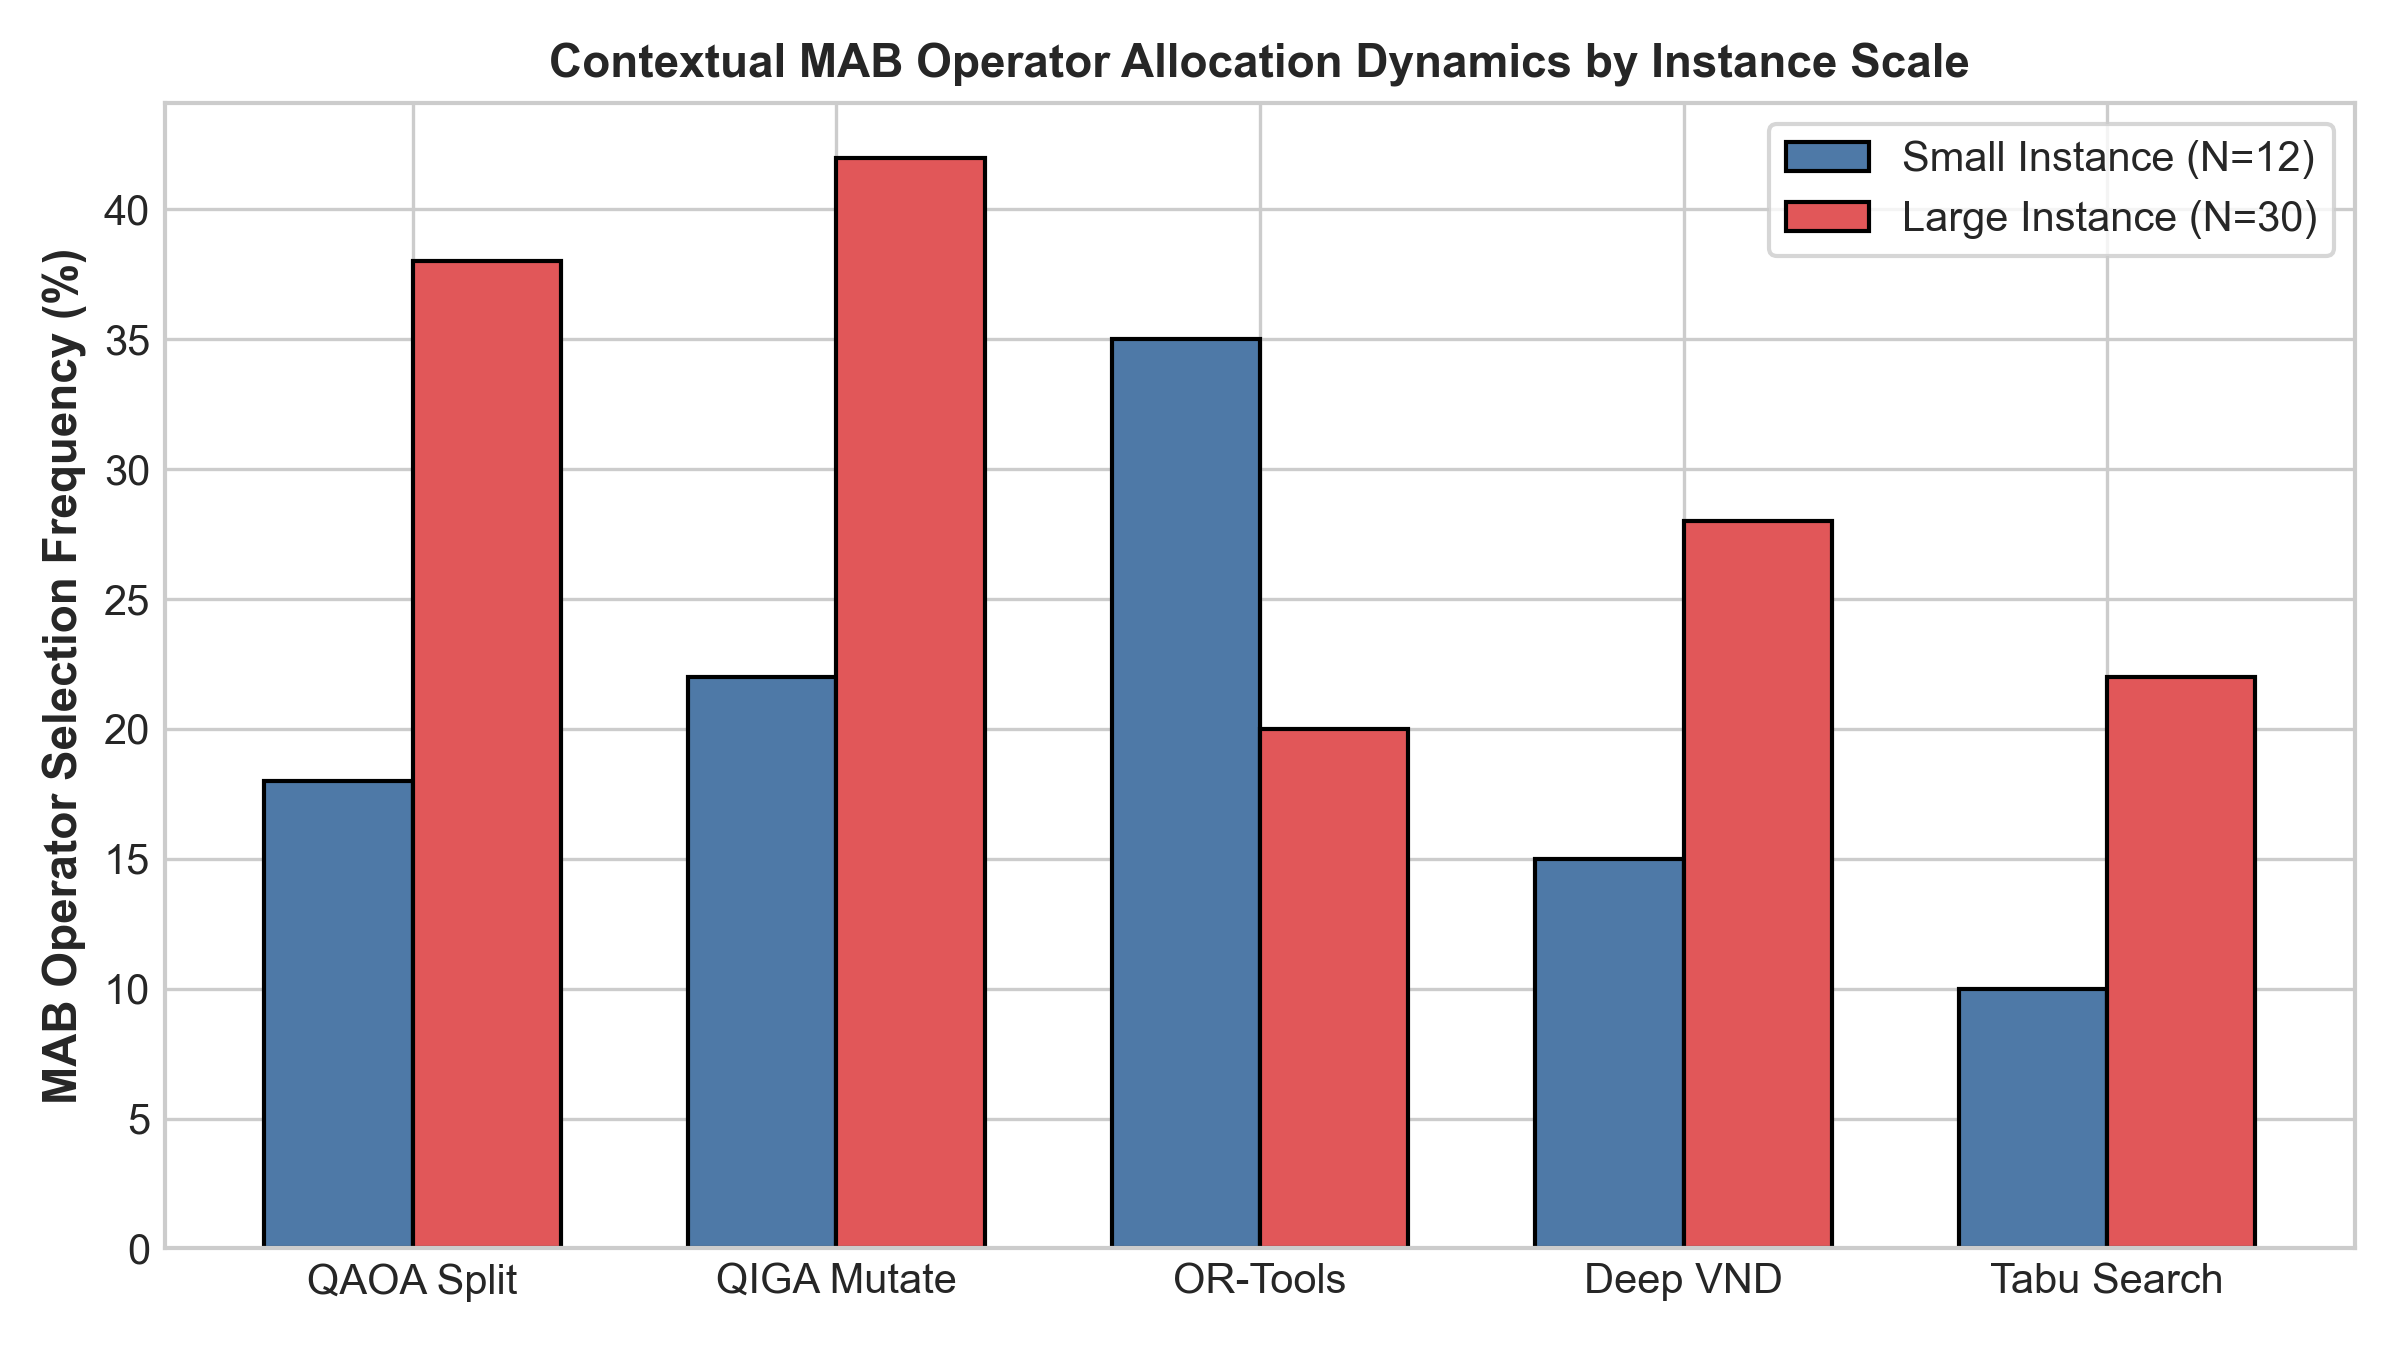
\includegraphics[width=0.48\textwidth]{figures/fig4_mab_operator_distribution.png}
\caption{Contextual MAB operator allocation dynamics across small ($N=12$) versus large ($N=30$) instance scales.}
\label{fig:mab_dist}
\end{figure}

\subsection{Ablation Analysis}
As detailed in Table~\ref{tab:ablation_study}, removing the candidate pool blackboard (Ablation 3) caused the mean distance to degrade by \textbf{+1.09\%} back to 181.26 km, proving that shared candidate exchange is the primary mechanism driving cooperative improvement. Removing QAOA or QIGA similarly restricted population diversity ($\mathcal{D}$ dropped from $0.54$ to $0.38$ and $0.35$).
